\documentclass{beamer}

\usepackage{tikz}
\usetikzlibrary{mindmap,trees}

\begin{document}

% -------------------------------------------
\begin{frame}
    %\frametitle{This is the first slide}
\begin{center}
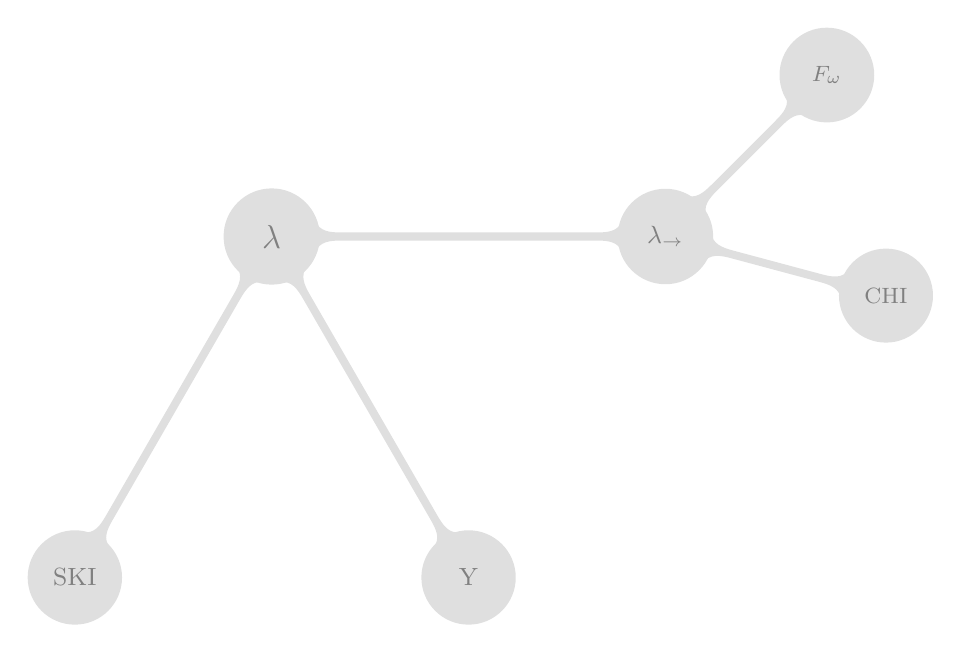
\begin{tikzpicture}
\path[mindmap, 
      concept color=lightgray!50!white,text=gray,
      every node/.style={minimum size=0pt,text width=30pt}]
    node[concept] {$\lambda$}
    [clockwise from=0]
    child[concept] {
      node[concept] {$\lambda_\rightarrow$}
      [clockwise from=45]
      child { node[concept] {$F_\omega$} }
      child { node[concept] {CHI} }
    }  
    child[concept] { node[concept] {Y} }
    child[concept] { node[concept] {SKI} };
\end{tikzpicture}
\end{center}
\end{frame}
% -------------------------------------------
\begin{frame}
\begin{center}
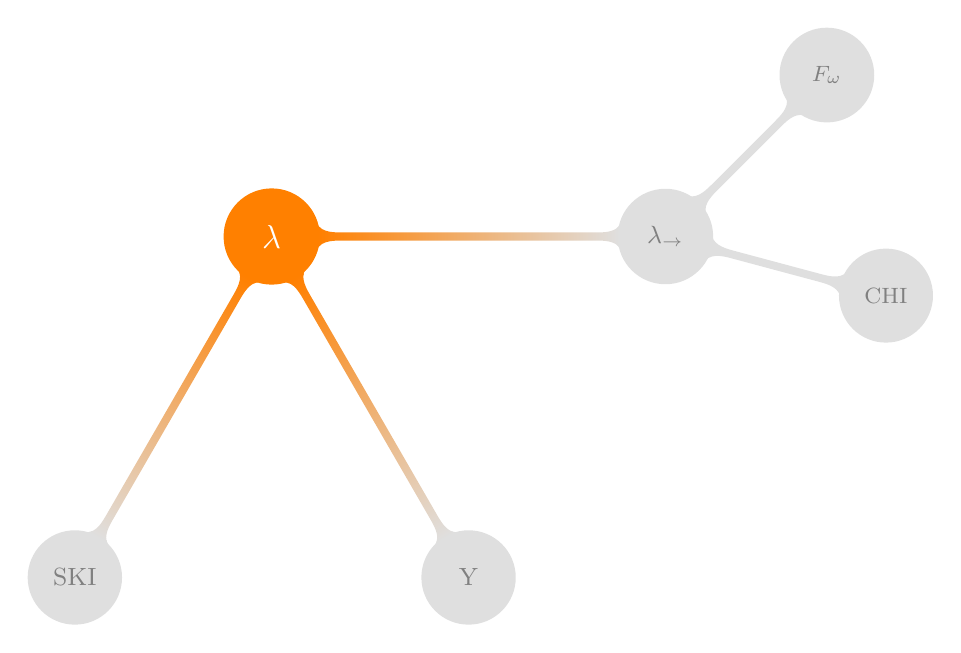
\begin{tikzpicture}
\path[mindmap, 
      concept color=orange,text=white,
      every node/.style={minimum size=0pt,text width=30pt}]
    node[concept] {$\lambda$}
    [clockwise from=0]
    child[concept color=lightgray!50!white,text=gray] {
      node[concept] {$\lambda_\rightarrow$}
      [clockwise from=45]
      child { node[concept] {$F_\omega$} }
      child { node[concept] {CHI} }
    }  
    child[concept color=lightgray!50!white,text=gray] { node[concept] {Y} }
    child[concept color=lightgray!50!white,text=gray] { node[concept] {SKI} };
\end{tikzpicture}
\end{center}
\end{frame}
% -------------------------------------------
\begin{frame}
    \frametitle{This is the second slide}
    \framesubtitle{A bit more information about this}
    Some text
    %More content goes here
\end{frame}
\end{document}
